\chapter{Introduction}\label{chap:introduction}
In recent years there has been a large increase in so-called \emph{smart devices}. 
A smart device is an electronic device that is connected to one or more other smart devices. 
Common protocols for the interconnection of smart devices are WiFi or Bluetooth, among others.
Smart devices are part of a concept called the Internet of Things, or IoT. 
IoT is a network of physical devices, 
where the devices have unique identifiers and are connected to the Internet, 
making them accessible from other devices such as personal computers or smartphones. 
Example of devices that are part of a network could be an air condition unit, a coffee machine, a watch or a refrigerator. 
Devices such as smartphones, laptops or servers, 
that are already commonly connected to the Internet, 
are usually not considered part of the IoT network. 

We will in this chapter gain an insight of what is the current state of \emph{wearables} and \emph{smart homes}. 
We first describe the initial problem in \Cref{sec:initproblem}, 
that describes what information we are looking to explore and why. 
After describing this problem, we will analyze wearables, 
\ie smart devices that are worn, in \Cref{sec:wearables}.
Another large part of IoT is the concept of smart homes, 
\ie homes that are controlled or automated by utilizing smart technologies and devices. 
We will analyze smart homes in \Cref{sec:smarthomes}, 
where \Cref{sec:system-categories} describes different levels of home automation. 
Finally we propose a problem statement \Cref{sec:researchstatement}, 
and give an overview of the rest of the report in \Cref{sec:overview}.

\section{Initial Problem}\label{sec:initproblem}
Wearable technology is a trending form of technology as of 2015 \cite{WEARABLESTREND}. 
As the name implies, wearables are devices that, 
unlike most electronics, are worn by the user. 
As shown by \Cref{fig:wearables-placement}, 
the most common type of wearables today are wrist-worn, 
\eg smartwatches or smart-wristbands (such as fitness trackers).
Smartwatches are watches that run an advanced operating system, 
and can perform more actions than regular watches, 
such as communicating with a smartphone or other smart devices.
Smart-wristbands are typically fitness trackers which track activity, among other things, 
and send this data to a connected smartphone via an application. 
Smartphones are usually not considered a wearable since they are \emph{carried} and not \emph{worn}. 

\begin{figure}[!htb]
  \centering
  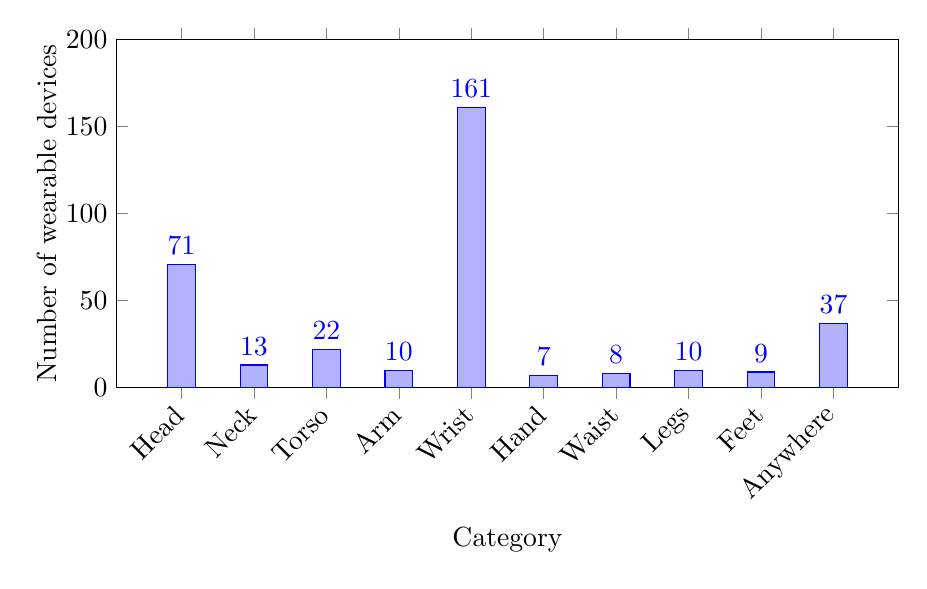
\begin{tikzpicture}
\begin{axis}[
    height=6cm,
    width=0.95\textwidth,
    xlabel={Category},
    xticklabel style={rotate=45, anchor=east, yshift=-0.5ex},
    ylabel={Number of wearable devices},
    yticklabel style={align=right,inner sep=0pt,xshift=-0.3em},
    nodes near coords align={vertical},
    nodes near coords,
    xtick=data,
    symbolic x coords={Head,Neck,Torso,Arm,Wrist,Hand,Waist,Legs,Feet,Anywhere},
    ybar,
    ymax=200,
    ymin=0,
    ]
    \addplot coordinates {(Head,71) (Neck,13) (Torso,22) (Arm,10) (Wrist,161) (Hand,7) (Waist,8) (Legs,10) (Feet,9) (Anywhere,37)};
\end{axis}
  

\end{tikzpicture}
  \caption{Placements of wearables. Data from \protect\cite{LISTOFWEARABLES}.}
  \label{fig:wearables-placement}
\end{figure}

The increasing trend in wearables is likely due to increased computational power in small devices, 
and decreased sizes of sensors, 
which allows more power and functionality to wearables devices. 
This increasing trend, as well as better wearables devices, 
opens up new possibilities since we can now carry more computational power with us on the go, 
which we can utilize to perform actions that we could not before, 
or perform actions faster or better. 
An example of this is that we can now track our level of activity, 
together with our location to analyze ourselves, 
or even automate actions based on our location, mood or even health. 

Another trend that utilizes IoT is smart homes.
Smart homes are homes that are to some degree automated by utilizing IoT devices. 
The devices used for smart homes differ from wearables as they are usually stationary. 
The concept of smart homes has been around since the 1960's, 
where ``wired homes'' were built by hobbyists\cite{harper2003}. 
The first official use of ``Smart house'' was in 1984, 
by the American Association of Housebuilders \cite{harper2003}.

An extreme example of a high-end smart home is Bill Gate's mansion in Medina, Washington \cite{billgatehouse}.
This \$100 million house, finished in 2005, 
has sensors to adjust each room's temperature and lighting, 
and has speakers behind the wallpaper that follow you from room to room. 
The artwork in the house is mostly digital and can be changed by pressing a button. 
One can only imagine what other technology is being used in that house. 

With these increasing technology trends in wearables and smart homes, 
it could be very interesting to see how and if we can integrate these. 
It could be interesting to see if we can use wearables as a form of control of smart homes, 
or maybe even use wearables to automate the smart homes.
In the following sections we will look into the current state of wearables and smart homes, 
and investigate if we can integrate them. 

\section{Wearables}\label{sec:wearables} %Working title
%Thalley: Første source kan også laves som en fin graf hvis ønsket. Brug tal fra: http://www.statista.com/statistics/259372/wearable-device-market-value/
Wearable technology is a trending form of technology as of 2015 \cite{WEARABLESTREND}. 
As the name implies, wearables are devices that, unlike most electronics, are worn by the user. 
The most common types of wearables today are smartwatches, 
\ie watches that run an advanced operating system and can perform more actions that regular watches such as communicating with a smartphone or other smart devices, 
and smart wristbands which usually tracks activity, 
among other things, and sends this data to a connected smartphone via an application. 
Smartphones are usually not considered a wearable since they are usually \emph{carried} and not \emph{worn}. 

%Hvorfor wearables?
The increasing trend in wearables is likely due to increased computational power in small devices and decreased sizes of sensors, 
which allows more power and functionality to wearables devices. 
The increasing trend, as well as better wearables devices, 
opens up new possibilities since we can now carry more computational power with us on the go that we can utilize to perform actions that we could not before, 
or perform other actions faster or better. 
Examples of this could be that we can now track our level of activity together with our location to analyze ourselves or even automate actions based on our location, mood or even health. 

%HVad kan en wearable? Hvilke sensorer findes der? Hvad er state of the art? 
If we take a look at some of the current state of the art or the most popular wearable devices right now, 
we can create an image of what we can actually monitor, track, control or in other ways do with devices that we can wear. 
One of the latest and most advanced wearable is the HIRIS \cite{hirisweb}. 
The HIRIS is a wearable computer able to track 3D movements in real-time. 
By using several HIRIS, you can get a create a full-body tracking system. 
Aside from 3D tracking, HIRIS also tracks heart rate and temperature and can connect to other devices and control these. 
Another advanced wearable tracker is the Jawbone UP3 \cite{JAWBONE}. 
This wearable is also able to track your heart rate, activity, sleep and temperature, but unlike the Hiris cannot control any other devices. 
Since one of the most popular wearables is the smartwatch, it makes sense to mention these as well. 
One of most interesting smartwatches, due to developer options, is the Pebble Smartwatch \cite{PEBBLE}. 
This smartwatch works with iPhones and Android smartphones and comes with a variety of applications for tracking fitness and control music among other things. 
Aside from this, the watch also comes with an accelerometer and a magnetometer, meaning that is can track your motions and directions. 

By analyzing the list of 348 different wearables from Vandrico\cite{LISTOFWEARABLES} of September 2015, 
we can see which sensors and components are most common among wearables and where on the body they are worn. 
It is important to note that all of this information comes Vandrico's database, and may differ from other findings. 
\Cref{fig:wearables-category} shows which categories these wearables fit in. The most common one, lifestyle, 
describes wearables such as smartwatches or other devices that are meant to be used and worn on a daily basis. 
Some devices may fit more than one category.

\begin{figure}[!htb]
    \centering
    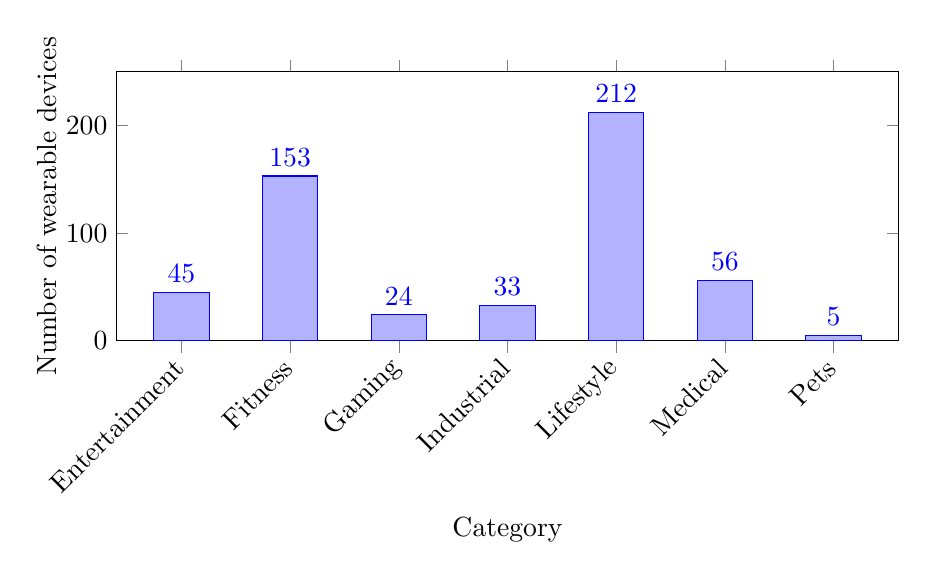
\begin{tikzpicture}
    \begin{axis}[
        height=5cm,
        width=0.95\textwidth,
        xlabel={Category},
        xticklabel style={rotate=45, anchor=east, yshift=-0.5ex},
        ylabel={Number of wearable devices},
        yticklabel style={align=right,inner sep=0pt,xshift=-0.3em},
        nodes near coords align={vertical},
        nodes near coords,
        xtick=data,
        symbolic x coords={Entertainment,Fitness,Gaming,Industrial,Lifestyle,Medical,Pets},
        ybar,
        ymax=250,
        ymin=0,
        bar width=20pt,
        ]
        \addplot coordinates {(Entertainment,45) (Fitness,153) (Gaming,24) (Industrial,33) (Lifestyle,212) (Medical,56) (Pets,5)};
    \end{axis}
\end{tikzpicture}
    \caption{Number of devices in each category}
    \label{fig:wearables-category}
\end{figure}

\Cref{fig:wearables-placement} shows where on the body the wearable should or can be worn. 
The most common placement is the wrist where smartwatches or wristband are worn, 
which are the most popular wearables. The devices that are worn on the head are usually augmented/virtual reality headsets, 
but also includes smart bike-helmets or ear/headphones.

\begin{figure}[!htb]
  \centering
  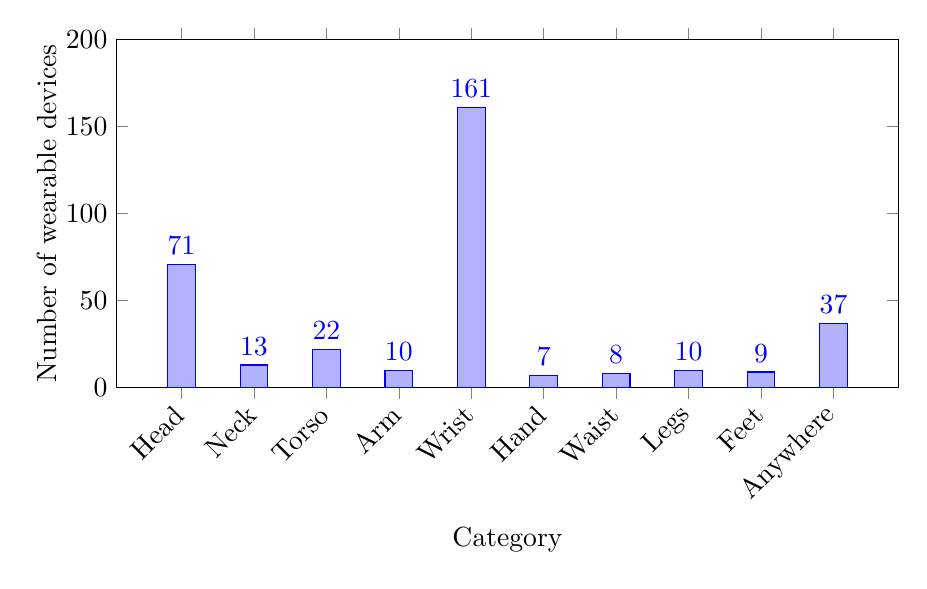
\begin{tikzpicture}
\begin{axis}[
    height=6cm,
    width=0.95\textwidth,
    xlabel={Category},
    xticklabel style={rotate=45, anchor=east, yshift=-0.5ex},
    ylabel={Number of wearable devices},
    yticklabel style={align=right,inner sep=0pt,xshift=-0.3em},
    nodes near coords align={vertical},
    nodes near coords,
    xtick=data,
    symbolic x coords={Head,Neck,Torso,Arm,Wrist,Hand,Waist,Legs,Feet,Anywhere},
    ybar,
    ymax=200,
    ymin=0,
    ]
    \addplot coordinates {(Head,71) (Neck,13) (Torso,22) (Arm,10) (Wrist,161) (Hand,7) (Waist,8) (Legs,10) (Feet,9) (Anywhere,37)};
\end{axis}
  

\end{tikzpicture}
  \caption{Placements of wearables}
  \label{fig:wearables-placement}
\end{figure}

\Cref{fig:wearables-sensors} shows which sensors and components are mostly available in wearables. 
Due to its high usability, the accelerometer is a very important sensor which is found in approximately half the wearables. 
The remaining sensors in \Cref{fig:wearables-sensors} are, unsurprisingly sensors that we also find in smartphones as they give a lot of options when it comes to developing applications. 
\begin{figure}[!htb]
    \centering
    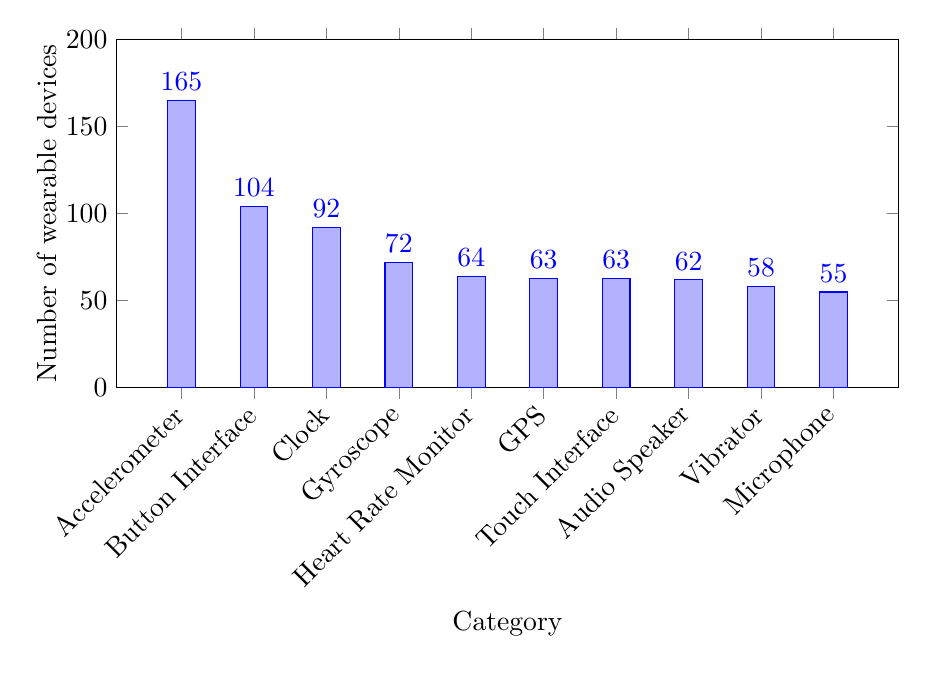
\begin{tikzpicture}
\begin{axis}[
    height=6cm,
    width=0.95\textwidth,
    xlabel={Category},
    xticklabel style={rotate=45, anchor=east, yshift=-0.5ex},
    ylabel={Number of wearable devices},
    yticklabel style={align=right,inner sep=0pt,xshift=-0.3em},
    nodes near coords align={vertical},
    nodes near coords,
    xtick=data,
    symbolic x coords={Accelerometer,Button Interface,Clock,Gyroscope,Heart Rate Monitor,GPS,Touch Interface,Audio Speaker,Vibrator,Microphone},
    ybar,
    ymax=200,
    ymin=0,
    ]
    \addplot coordinates {(Accelerometer,165) (Button Interface,104) (Clock,92) (Gyroscope,72) (Heart Rate Monitor,64) (GPS,63) (Touch Interface,63) (Audio Speaker,62) (Vibrator,58) (Microphone,55)};
\end{axis}
  

\end{tikzpicture}
    \caption{Top 10 mostly used sensors}
    \label{fig:wearables-sensors}
\end{figure}

This section gave a short overview of the current state of wearables, what they are and which sensors are widely available. 
This information should be remembered if developing any system that utilizes wearables. 

%Skab et overblik over de nyeste devices
%Grafer over hvilke sensorere der mest typiske?
%Grafer over kropsdele?
%Hvad er de nyeste teknologier indenfor wearables? 

\section{Smart Homes}
Another trend that utilizes the concept of IoT is smart homes which are homes that are, to some degree, automated by utilization IoT devices. 
The devices used for smart homes differ greatly from wearables as they are usually stationary. 
The concept of smart homes have been around for a while and numerous homes have already integrated some of these smart devices. 
A good example of a high-end smart home is Bill Gate's mansion in Medina, Washington \cite{billgatehouse}.
This \$100 million house have sensors to adjust each room's temperature and lighting and have speakers behind the wallpaper that follows you from room to room. 
The artwork in the house is mostly digital and can be changed by pressing a button. 
One can only imagine what other technology is being used in that house. 

However, that is a rather extreme example of a smart home. 
Ordinarily, the devices found in smart homes are common items that has been connected to the Internet for wireless control.
Common devices that are found in smart homes include, but are not limited to, 
coffee machines, washers and dryers, thermostats, sound systems and locks. 
However, only few devices have really gained ground for the common user and few homes are automated.
One of the most commonly found IoT in homes are the Nest thermostat \cite{NEST}. 
This thermostat senses when you are around and when you are not to control the climate inside to save energy and thus money.
Unlike a lot of smart devices that are made to make your life a little easier, such as an automated coffee machine, 
the Nest thermostat helps you save money which is likely the reason for it popularity. 
Furthermore, the newest version (as of October 2015) allows you to connect other IoT devices to the thermostat. 
The Nest thermostat is thus starting to solve what is probable the greatest problem with smart homes (and IoT in general) and why they have not become popular yet: Lack of interconnectivity between IoT devices. 

\subsection{Smart Hubs}
%Something about SmartThings
%How does wearables fit in

\subsection{Indoor Positioning}\label{sec:indoor-positioning}
%Something about Estimote
In order to determine which device the user points at and thereby intends to control, 
it is necessary to determine the locations of the devices in the system relative to the user.

The focus of this project is not to position devices and as such it was not the intention to spend time developing an entire solution for positioning devices indoors. 
Instead it was desired to find an existing product that could be used to facilitate indoor positioning.
The solution should be available in the early phases of the project in order to start building the system based on the solution for positioning.

Ideally users of this project should be able to control any device that fits within the concept of Internet of Things he owns, 
the price for any device needed to position each controllable device should be low. 
If a user owns several devices that can be controlled using gestures and an extra device is needed for each in order to preform the positioning, 
the price of such a device should be at a minimum.

It is assumed that users already own one or more devices that fit within the concept of Internet of Things and possibly are early adapters of such technology, 
it is assumed they have some technological expertise. 
However, it easy to imagine that this project can be used in an office environment where employees of varying technological expertise work or in health care. 
Therefore users may have a varying degree of technological expertise and it should be easy to extend the solution with new controllable devices.

Naturally the accuracy of the solution used for positioning objects plays an important part. 
\Cref{fig:indoor-positioning:incorrect} shows the consequence of an incorrect location. 
If a lamp is estimated to be at another location that it is actually located, 
the user must point to an incorrect location in order to control the lamp.
Furthermore if the estimate is too wide, that is, the given area in which the lamp is located is very big, 
there is a greater risk that locations overlap. 
Overlapping locations causes a complexity as it is necessary to determine which device the user desires to control if he points at the overlap as visualized in figure \ref{fig:indoor-positioning:overlap}.

\begin{figure}[h]
    \centering
    \includegraphics[height=5cm]{images/incorrect-positioning-estimate.png}
    \caption{Incorrect location estimate. The estimate is visualized as a striped circle.}
    \label{fig:indoor-positioning:incorrect}
\end{figure}

\begin{figure}[h]
    \centering
    \includegraphics[height=5cm]{images/positioning-overlap.png}
    \caption{Overlap of estimated positions. The estimates are visualized as a striped circle.}
    \label{fig:indoor-positioning:overlap}
\end{figure}

Based on the above the following criteria for assessing potential solutions can be outlined.

\begin{itemize}
    \item Availability
    \item Price
    \item Ease of use
    \item Accuracy
\end{itemize}

Only solutions intended for indoor positioning was considered and thus GPS is not considered a potential solution. 
GPS is meant for outdoor positioning and a signal is not always available while indoors and even if it is, the accuracy of the estimated location is very low.

\begin{table}[h]
    \centering
    \caption{Assessment of potential solutions for indoor positioning. Please not that all prices are converted to U.S. dollars from their respective currency. Prices include the minimum available hardware for positioning a device.}
    \label{tbl:indoor-positioning}
    
    \begin{tabularx}{\textwidth}{XXXXX}
        \textbf{Product} & \textbf{Availability} & \textbf{Price} & \textbf{Ease of use} & \textbf{Accuracy} \\
        
        Estimote Beacons and Stickers \cite{estimote}
        & Beacons and Stickers are shipping. SDKs available.
        & \$99 for beacons. \$99 for 10 stickers, one per device to be positioned.
        & Initial installation of beacons. Attach each sticker to device.
        & Unknown. Desired to be less than five meters. \todo[author=Simon]{Update after conducting tests.} \\
        
        Pozyx \cite{pozyx}
        & Available for preorder.
        & \$368 for anchors. \$123 for each device to be positioned, plus supported Arduino.
        & Initial installation of anchors. One tag for each device, plus supported Arduino. Not meant for mounting.
        & Claimed to be 10 cm. Untested.
        
    \end{tabularx}
\end{table}

%%% Local Variables:
%%% mode: latex
%%% TeX-master: "../../master"
%%% End:

\section{System Categories}\label{sec:system-categories}
Smart home automation is one of the big sell-points of smart homes.
Home automation can happen at various degrees. 
In this section we will analyze and categorize the different types of smart home automation. 

The scenarios in which home automation is facilitated can in general be divided into the following three categories.

\begin{enumerate}
    \item Rule driven systems
    \item Gesture driven systems
    \item Autonomous systems
\end{enumerate}

The categories varies in the way users configure and interact with the systems. 
``Manual systems'' could constitute a fourth category, consisting of regular systems with manual switches,
but is left out as it such systems do not contribute to home automation.
Each of the three categories and their use cases are briefly described below.

\subsection{Rule Driven Systems}

A system is considered to be rule driven if an action is executed when a set of rules are fulfilled. 
The rule driven systems use conditional statements to express input and output. 
Below are a few examples of rules in the form of (if this) \textrightarrow (then that):

\begin{itemize}
    \item (The temperature is above 23 degrees Celsius) \textrightarrow~(Lower the temperature on my thermostat)
    \item (The CO\textsubscript{2} index is critically high) \textrightarrow (Open my windows)
\end{itemize}

The above rules consist of a condition on the left-hand side of the arrow and an action on the right-hand side of the arrow.
The automation of the smart home is based on the set of rules. 
To achieve the desired behavior, the user must add, remove or tweak existing rules.

Examples of rule drive systems include the aforementioned Apple HomeKit. 
As outlined in the framework reference for HomeKit \cite{applehomekitref}, the system is based on actions and events. 
Triggers constitutes rules by encapsulating actions and events. 
Each event represents a condition. 
An event may be fulfilled by a change in time, the state of devices in the system of the location of the user.

\subsection{Gesture Driven Systems}

Systems are gesture driven if the system is configured with a set of gestures that can be performed by the user in oder to trigger some action. 
Each device in the system responds to a set of gestures. 
For example, a lamp may respond to the user waving in order to turn on and the user clapping in order to turn off.

A gesture driven system is partly rule driven as each gesture registered in the system is associated with one or more actions. 
The association means that each time the gesture is registered in the system, the action should be triggered. 
Such rules can be formulated as ``if I wave, then lower the temperature on my thermostat''

Examples of gesture driven systems includes Hiris, a wearable computer with focus on gestures that allow the users to interact with other devices \cite{hirisweb}.

\subsection{Autonomous Systems}

An autonomous system monitors the system and proactively responds to changes in the system. 
Observable changes include but are not limited to changes in the temperature, CO\textsubscript{2} index, the number of people in the room or even who are in the room.
Autonomous systems should intelligently react to the users needs based upon the observable state of the environment.

Autonomous systems rely on the concept of ambient intelligence in order to determine the necessary actions.
\todo[author=Thalley]{Maybe add something about ambient intelligence here?}
Such systems include autonomous enhancement services that replaces manual care with an automated system \cite{nehmer2006living}. 
These systems gather environment and the data about the individuals body functions, 
\eg temperature, pulse and blood pressure in order to determine if the individuals health is critical.

Autonomous systems are rule driven systems that intelligently determines the rules to be created and the necessary action to take when a set of rules are fulfilled. 
Typical for such systems may be the complexity of the rules. 
It is not given that users themselves are capable of determining a suitable set of rules in order to judge if their health is critical. 
The system should itself be able to determine such set of rules and adjust it to the individual.

Examples of autonomous systems include the one described Nehmer \etal\cite{nehmer2006living}. 
The authors envision a living assistance system which monitors elderly people. 
A model is outlined and by continuously feeding the model with data about the individuals body functions and his behavior, 
they can determine if a \emph{critical situation} occurs. 
A critical situation could be that the person has fallen and are not responding to contact, for example calls.
Such system may reduce the cost of providing care to the elderly people.

\subsection{Conclusion}

The rule driven, gesture driven and autonomous systems are all rule driven to some extend but the origin and the types of rules differ between the systems. 
In a rule driven system the rules are configured by the user.
In an autonomous system the rules are programmed by some expert or in collaboration with experts in a certain field, \eg the medical field. 
The system may adapt its set of rules based on the environment and that behavior of the individual.
Gesture driven systems use rules configured by the user. 
In such systems gestures make up the condition of a rule.

When concerned with the field of home automation it is relevant to classify each system in order to determine how automatic a system is. 
The more automatic a system is, the less the user should be involved with the system.

The degree of automation as well as the reasoning behind each of the classifications are shown in \Cref{tbl:system-categories}.

\begin{table}[h]
    \centering
    \begin{tabularx}{\textwidth}{XXX}
    \textbf{Gesture driven systems}       & \textbf{Rule driven systems}                             & \textbf{Autonomous systems} \\
    \textit{Lowest degree of automation}  & \textit{Medium degree of automation}                     & \textit{Highest degree of automation}\\
    Configured by the user.               & Configured by the user.                                  & Configured by an expert.\\
    Conditions are triggered by the user. & Automatically and constantly observes the environment.   & Automatically and constantly observes the environment.\\
    ~                                     & The configuration may be reusable for other individuals. & Automatically adjusts to the users needs.\\
    \end{tabularx}
    \caption{Classification of systems based on their degree of automation}
    \label{tbl:system-categories}
\end{table}

%%% Local Variables:
%%% mode: latex
%%% TeX-master: "../../master"
%%% End:

\section{Problem Statement}
In the previous sections we analyzed different areas of Internet of Things (IoT) including how wearables and home automation are maturing. 
We have seen some of the possibilities of wearables and we can see that this can integrated with home automation and indoor location.
We think that exploring the concept of home automation with wearables can result in a usable system that better utilizes the devices for smart homes by giving a better interface. 
More accurately, we want to explore the possibilities of interconnecting smart devices using existing technologies.
In the remainder of this report, we will answer the following question:
\begin{framed}
    \begin{quote}
        What can we do with wearables and smart devices in a smart home setting, where different smart devices may use different communication protocols?
        
        In answering this question, we will also answer the following questions:
        \begin{itemize}
            \item What problems arise when working with different platforms using different operating systems?
            \item Which limitations does current technology have in the area of IoT? Can we overcome it and how? 
           \end{itemize} 
    \end{quote}
\end{framed}
%Thalley: For meget med frame? Evt. bruge noget andet for at fremhæve problemformuleringen, eller bare droppe det helt? 


%Thalley: Gammel formulering:
%\begin{quote}
%    \begin{itemize}
%        \item Explore the possibilities of interconnecting smart devices using existing technologies  
%        \item Give users a better interface of controlling smart devices with gestures using a wearable in a smart home 
%    \end{itemize}    
%\end{quote}
%
%The goal of our research is to create a system that allows gesture-based communication between the user and smart devices.
%We feel that allowing users to point and control devices will give the best interface. 
%This approach requires accurate indoor location, a wearable that can recognize gestures and a hub for interoperability between the wearable and the smart devices. 
%!TeX root = ../../master.tex
\section{Requirements Specification}
\label{sec:requirements-specification}

In this section we will list the requirements that the system we develop must fullfil.

\subsection{Users should be able to set up a room}
The user needs to be able to specify the positions of the Estimote beacons in a room, as well as the shape and size of the room. They should be able to do this for multiple rooms so they can use the system in their entire home.

\subsection{Users should be able to add smart items to a room}
If the user is performing a first time setup or has acquired a new smart item in his home, he needs to be able to add it to the room.

\subsection{Users should be able to specify the position of a smart item by using his own position}
The user should be able to configure a position of a smart item by standing next to it and clicking an ``Assign Location'' button.

This is needed first time the user adds a smart item to a room, but also when a smart item is moved or removed.

\subsection{Users should be able to create their own gestures}
The user needs to be able to create new gestures and train them.

\subsection{Users should be able to assign a gesture to an action}
The user should be able to link a gesture to a certain action, eg. \textit{Clockwise circle} turns up the stereo.

\subsection{Users should be able to control smart items by pointing at them and performing a gesture}
The system needs to detect when a user is pointing at smart items, determine which items are being pointed at and react to any gestures performed.


\section{Overview}\label{sec:overview}
This section will briefly describe the structure and the content of rest of the report. 
This report consists of 6 chapters and should be read from Chapter 1 through Chapter 6. 
The first chapter, \Cref{chap:introduction}, which you have just read, 
was an introduction to the problem domain, 
briefly exploring existing technologies in the area of IoT. 
In \Cref{chap:analysis} we further analyze the problem, 
and existing solutions.
\Cref{chap:design} describes the architecture and design of our system. 
The system's implementation, and prototypes during the project, 
will be described in \Cref{chap:implementation}.
Then we evaluate our system in \Cref{chap:evaluation}, 
to see if it meets the requirements from \Cref{sec:requirements-specification}.
Lastly, we end this report by making a conclusion in \Cref{chap:conclusion}, 
where we show and discuss the final results, 
and discuss how the system may be further improved. 

